\subsection{Rust}
Rust е програмен език от високо ниво създаден през 2006 година от Graydon
Hoare, който по това време работи за Mozilla. През 2009 година разработката на
езика бива спонсорирана от Mozilla, a през 2010 езика е обявен публично.
\cite{Rust_Origins_Wikipedia}

\subsubsection{Отличаващи се особености на езика}
% Rust е порграмен език от високо ниво, но това не му пречи да е почти толкова
% бърз колкото езици от по-ниско ниво като C/C++.

Езици като C\#, Python и JavaScript използват система за освобождаване на паметта
наречена Garbage Collector (GC). За да може да се освободят неизползваните
променливи, изпълнението на програмата трябва да бъде спряно на пауза и да се
провери дали има заделени региони от паметта, към които вече не се използват
или са маркиране за освобождаване от програмиста \cite{Garbage_Collection_Wikipedia}.

Rust използва система наречена borrow checker, която проверява, по време на
компилация, дали програмата следва следните принципи:

\begin{itemize}

\item Ресурсите (отделената памет за стойноста) могат да имат само един
собственик и това е самата промелива. Когато променлива вече не може да бъде
достъпена ресурсите биват освободени.

\item Когато една променлива бъде подадена към някоя функция, собственик на
ресурсите става функцията. Ако се пробваме подадем отново променливата,
компилатора ще ни каже, че променливата е била преместена (Use of moved value).
\begin{figure}[!htb]
  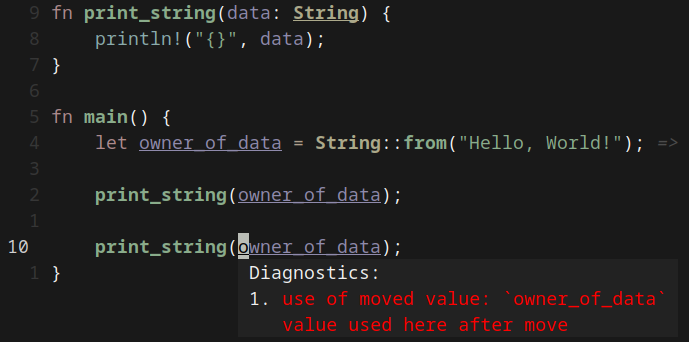
\includegraphics[width=\textwidth,keepaspectratio=true]{rust-use-after-move}
  \centering
  \caption{Модела на собственик в Rust}
  \label{fig:rust-use-after-move}
\end{figure}

\end{itemize}

\subsubsection{Enum}
Enum е един от основните типове в Rust. Всеки вариянт на enum-а може да има
съдържа информация от различен вид \cite{Rust_Enums}. Така са имплементирани
някои от най-важните типове: Option<T> и Result<T, E>.

\begin{figure}[!htb]
  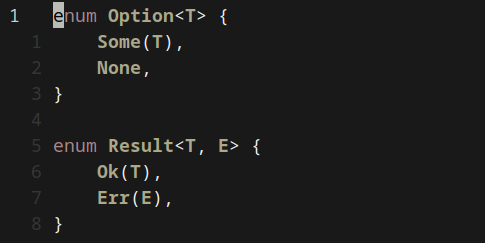
\includegraphics[scale=0.75]{rust-enum-example}
  \centering
  \caption{Стандартната имплементация на Option<T> и Result<T, E>}
  \label{fig:rust-enum-example}
\end{figure}

\subsubsection{Option типа}
В повечето езици съществува идеята за NULL пойнтери. Когато един pointer е Null
това означа, че той сочи към нищо. Идеята за Null на теория е много добра, но
на практика създава повече проблеми. Ако се пробваме да достъпим pointer който
е Null, програмата ще крашне или в някои езици като C\# ще хвърли
NullReferenceException.

Разработчиците на Rust са намерили много добър заместител на Null и това е
Option enum-а, който има два варинта. Това са Some(T), когато имаме някаква
стойнос и None, когато нямаме нищо.

\subsubsection{Result типа}
Когато програмираме на C\# много често ни се случва да хвърляме Exception-и и
съответно да ги хващаме с try/catch блока. Еxception-ите се ползват, когато в
една функция възникне грешка.

Във Фигура \ref{fig:csharp-exceptions-1-code} е даден код, който на пръв поглед
изглежда добре, но има скрити бъгове. Какво ще стане, ако потребилтелят въведе
дума вместо число? Ще получим Exception, който ни казва: "Input string was not
in a correct format".
\begin{figure}[!htb]
  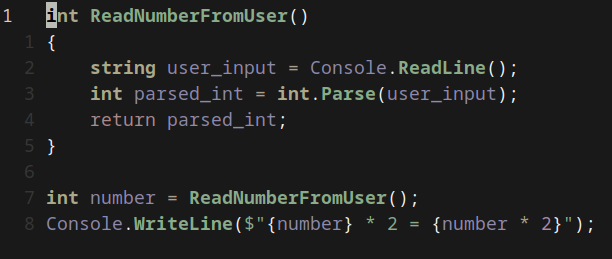
\includegraphics[scale=0.75]{csharp-exceptions-1-code}
  \centering
  \caption{Пример за скрит Exception}
  \label{fig:csharp-exceptions-1-code}
\end{figure}


\begin{figure}[!htb]
  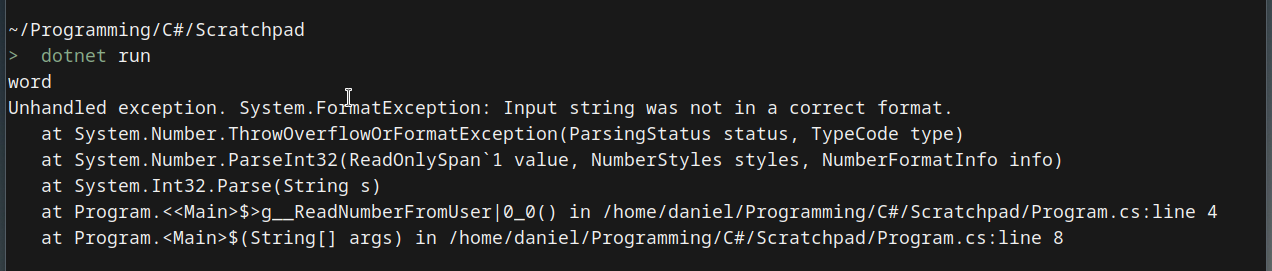
\includegraphics[width=\textwidth,keepaspectratio=true]{csharp-exceptions-1-output}
  \centering
  \caption{Изход на кода от Фигура \ref{fig:csharp-exceptions-1-code}}
  \label{fig:csharp-exceptions-1-output}
\end{figure}

Проблемът, е че ние като програмисти не знаем, че int.Parse може да хвърли
Exception без да се консултираме с документацията \cite{CSharp_Int_Parse}.
Същият код написан на Rust би изглеждал по следния начин [Фигура \ref{fig:rust-exceptions-1-code}].

\begin{figure}[!htb]
  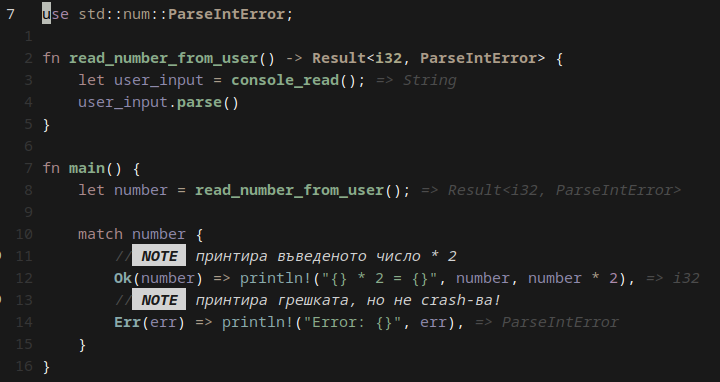
\includegraphics[scale=0.60]{rust-exceptions-1-code}
  \centering
  \caption{Кода от Фигура \ref{fig:csharp-exceptions-1-code} написан на Rust}
  \label{fig:rust-exceptions-1-code}
\end{figure}

Разликата между C\# и Rust, е че Rust кода ни показва типовете при успех
и грешка. Функцията връща променлива от тип Result<T, E>, където T е
променливата от тип i32 (int), ако всичко се и изпълнило без проблем, а E е от
тип ParseIntError.

За да използваме резултата от функцията, какъвто и да е той, можем да
използваме match. С match можем да проверим дали резултата е Ok или Err.
